% --------------------------------------------------------------
% This is all preamble stuff that you don't have to worry about.
% Head down to where it says "Start here"
% --------------------------------------------------------------
 
\documentclass[12pt]{article}
 
\usepackage[margin=1in]{geometry} 
\usepackage{amsmath,amsthm,amssymb,scrextend}
\usepackage{fancyhdr}
\usepackage{enumitem}
\usepackage{amsmath}
\usepackage{amssymb}
\usepackage{textcomp}
\usepackage{fancybox}
\usepackage{tikz}
\usepackage{tasks}
\pagestyle{fancy}
\usepackage[makeroom]{cancel}
\usepackage{graphicx}
\usepackage{caption}
\usepackage{mwe}
\usepackage{tikz}
\usetikzlibrary{positioning}

\newcommand{\N}{\mathbb{N}}
\newcommand{\Z}{\mathbb{Z}}
\newcommand{\I}{\mathbb{I}}
\newcommand{\R}{\mathbb{R}}
\newcommand{\Q}{\mathbb{Q}}
\renewcommand{\qed}{\hfill$\blacksquare$}
\let\newproof\proof
\renewenvironment{proof}{\begin{addmargin}[1em]{0em}\begin{newproof}}{\end{newproof}\end{addmargin}\qed}
% \newcommand{\expl}[1]{\text{\hfill[#1]}$}
 
\newenvironment{theorem}[2][Theorem]{\begin{trivlist}
\item[\hskip \labelsep {\bfseries #1}\hskip \labelsep {\bfseries #2.}]}{\end{trivlist}}
\newenvironment{lemma}[2][Lemma]{\begin{trivlist}
\item[\hskip \labelsep {\bfseries #1}\hskip \labelsep {\bfseries #2.}]}{\end{trivlist}}
\newenvironment{problem}[2][Problem]{\begin{trivlist}
\item[\hskip \labelsep {\bfseries #1}\hskip \labelsep {\bfseries #2.}]}{\end{trivlist}}
\newenvironment{exercise}[2][Exercise]{\begin{trivlist}
\item[\hskip \labelsep {\bfseries #1}\hskip \labelsep {\bfseries #2.}]}{\end{trivlist}}
\newenvironment{reflection}[2][Reflection]{\begin{trivlist}
\item[\hskip \labelsep {\bfseries #1}\hskip \labelsep {\bfseries #2.}]}{\end{trivlist}}
\newenvironment{proposition}[2][Proposition]{\begin{trivlist}
\item[\hskip \labelsep {\bfseries #1}\hskip \labelsep {\bfseries #2.}]}{\end{trivlist}}
\newenvironment{corollary}[2][Corollary]{\begin{trivlist}
\item[\hskip \labelsep {\bfseries #1}\hskip \labelsep {\bfseries #2.}]}{\end{trivlist}}
 
\setlength{\parindent}{0pt}
\begin{document}
 \settasks{
	counter-format=(tsk[r]),
	label-width=4ex
}
% --------------------------------------------------------------
%                         Start here
% --------------------------------------------------------------

\lhead{Math 632}
\chead{Homework 7}
\rhead{Meenmo Kang}
1.Three children take turns shooting a ball at a basket. They ea
ch shoot until they miss and then it is next child’s turn. Suppose that child $i\;(1\le i \le 3)$ makes a basket with probability $p_i$ and that successive trials are independent. Use the following two approaches to determine the average fraction of time in the long run that child $i$ shoots.
\begin{enumerate}[label=(\alph*)]
    \item (first method) Consider the renewal process with interarrival times $t_k = s_k^1 + s_k^2 + s_k^3,$ where $s_k^i$ is the number of shots child $i$ takes in the $k^{th}$ turn. Find $P(s_k^i = n)$. Then use this to compute the long run fraction of time child $i$ spends shooting the ball.
    
    \vspace{1\baselineskip}
    $$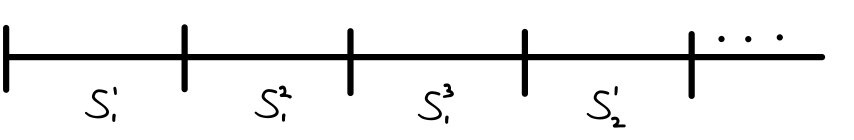
\includegraphics[height=1.5cm, width=10cm]{q1.jpeg}$$
    Since each trial is independent, the probability a kid $s^i$ makes $n$ shots for $k^{th}$ turn is 
    $$P(s_k^i=n) = p_i^{n-1}\cdot (1-p_i)\qquad
    Es_k^i = \sum\limits_{n=1}^\infty np_i^{n-1}(1-p_i)=\frac{1}{1-p_i}\;\;(\because \text{Geometric})$$
    $$Et_k = \frac{1}{1-p_1}+\frac{1}{1-p_2}+\frac{1}{1-p_3}
    $$
    \vspace{1\baselineskip}
    The long run fraction of time child $i$ spends shooting the ball:
    $$\lim\limits_{t\to\infty}\frac{1}{t}\sum\limits_{i=1}^{N(t)} s_k^i = \frac{Es_k^i}{Et_i} =
    \frac{\frac{1}{1-p_i}}   {\frac{1}{1-p_1}+\frac{1}{1-p_2}+\frac{1}{1-p_3}}
    =\frac{1-p_i}{\sum\limits_{i=1}^3 \frac{1}{1-p_i}}$$
    
    
    

    \item (second method) Consider the discrete time Markov chain with three states, where the system is in state $i\in S = \{1,2,3\}$ if child $i$ has the ball. Use the theory from chapter 1 to determine the long run fraction of time child $i$ spends shooting the ball.
    
    Markov Chain Matrix P
    $$P=\begin{bmatrix}
    p_1&1-p_1&0\\0&p_2&1-p_2\\1-p_3&0&p_3
    \end{bmatrix}$$
    
   Through the stationary distribution we can obtain $\pi$ such that $P=\pi P$.
   $$\pi = \left(\frac{\frac{1}{1-p_1}}{\sum\limits_{i=1}^3 \frac{1}{1-p_i}},\; \frac{\frac{1}{1-p_2}}{\sum\limits_{i=1}^3 \frac{1}{1-p_i}},\; \frac{\frac{1}{1-p_3}}{\sum\limits_{i=1}^3 \frac{1}{1-p_i}}    \right)$$
   
   $\pi_{1,2,3}$ is the long run fraction of time child $i$ spends shooting the ball.
\end{enumerate}

\newpage
2. A young doctor is working at night in an emergency room. Emergencies come in at times of a Poison process with rate 0.5 per hour. The doctor can only get to sleep when it has been 36min (0.6h) since the last emergency. For example, if there is an emergency at 1:00 and a second one at 1:17 then she will not be able to get to sleep until at least 1:53, and it will be even later if there is another emergency before that time.
$$t_i\sim \exp(0.5), \quad r_i:\text{ the amount of sleep for $i^{th}$ cycle}\; \begin{cases}t_i - 0.6&t_i > 0.6\\0&t_i\le 0.6 \end{cases} $$
$$R(t) = \sum\limits_{i=1}^{N(t)} r_i = \text{the amount of  sleep in the cycles completed by time $t$}$$
%$$S(t)=\text{the amount of sleep up to time $t$}$$

\begin{enumerate}[label=(\alph*)]
    \item Compute the long-run fraction of time she spends sleeping, by formulating a renewal reward process in which the reward in the $i$th interval is the amount of time she gets to sleep in that interval.
    $$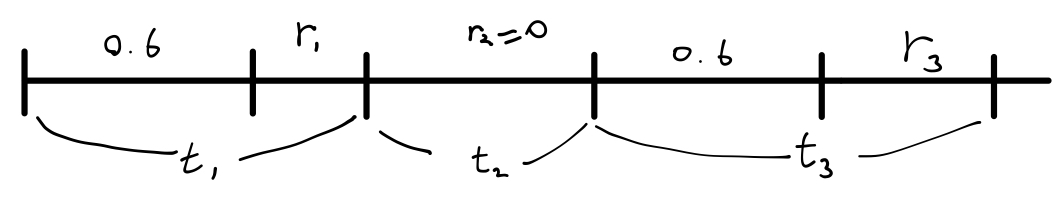
\includegraphics[height=1.5cm, width=10cm]{q2.jpeg}$$

\begin{align}
    E[r_1] = E[(t_1-0.6)^+] &= \int_0^\infty (t-0.6)^+\; 0.5e^{-0.5t}dt \nonumber \\
    &=\int_{0.6}^\infty (t-0.6)\;0.5e^{-0.5t}dt \tag*{\begin{cases} x=t-0.6 \\dt = dx\end{cases}} \\
    &=\int_0^\infty x\cdot 0.5 e^{-0.5(x+0.6)}dx
    = e^{-0.3}\int_0^\infty x\cdot 0.5 e^{-0.5 x}dx\nonumber \\
    &=e^{0.3}E[t_1] = 2e^{0.3} \nonumber \\
    &\Rightarrow \frac{E[r_1]}{E[t_1]} = \frac{2e^{-0.3}}{2} = e^{-0.3} \nonumber
\end{align}
    
    \item The doctor alternates between sleeping for an amount of time $s_i$ and being awake for an amount of time $u_i$. Use the result from (a) to compute $Eu_i$.
    
    \vspace{1\baselineskip} 
    Long-run fraction: Suppose $c_i = u_i + s_i$ 
    $$\lim\limits_{t\to\infty} \frac{s(t)}{t} = \frac{E[s_1]}{E[c_1]} = \frac{E[s_1]}{E[u_1]+\underbrace{E[s_1]}_{E[\exp(0.5)]}} = \frac{2}{E[u_1]+2} = \underbrace{e^{-0.3}}_{(a)}\quad\Leftrightarrow\quad E[u_1] = 2^{0.3}-2$$
    
\end{enumerate}


\newpage
3. While visiting Haifa, Sid Resnick discovered that people who wish to travel from the port area up the mountain frequently take a shared taxi known as a sherut. The capacity of each car is 5 people. Potential customers arrive according to a Poisson process with rate $\lambda$. As soon as 5 people are in the car, it departs for the Carmel, and another taxi moves up to accept passenger so on. A local resident (who has no need of a ride) wanders onto the scene. What is the distribution of the time he has to wait to see a cab depart?\\

$Hint.$ Letting $Z$ denote the time until the onlooker sees a cab depart, find the density function $g$ and the mean of $Z$. Compute the mean two ways: by (3.10) in Durrett, and by integrating with the density function $g$ you found for $Z$, and this way confirm your answer. Assume that when the person comes to observe, the process has been running for a long time.

\vspace{1\baselineskip}
$$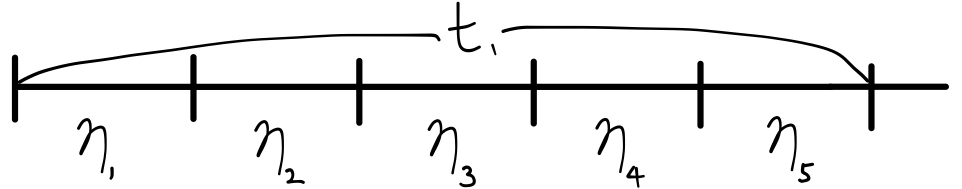
\includegraphics[height=1.5cm, width=10cm]{q3.jpeg}$$
$$g(z) = \frac{P(t_i>z)}{E[t_i]} = \frac{P(N(z)\le 4)}{E[t_i]}\qquad t_i = \sum\limtis_{i=1}^5 \eta_i \Rightarrow E[t_1] = 5E[\eta_1] = \frac{5}{\lambda}$$
$$g(z) = \frac{\lambda}{5}\left[e^{-\lambda z}\left(1+\lambda z+\frac{(\lambda z)^2}{2!}+\frac{(\lambda z)^3}{3!}+\frac{(\lambda z)^4}{4!}\right)\right]$$
$$E[z] = \frac{E[t_1^2]}{2E[t_i]} \qquad Var[t_i] = E[t_1^2]-(E[t_i])^2$$
$$E[t_i^2] = 5Var(\eta_1)+(E[t_i])^2 = \frac{5}{\lambda^2}+\frac{25}{\lambda^2} = \frac{30}{\lambda^2}\qquad\Rightarrow\qquad E[z] = \frac{30/\lambda^2}{2\times 5/\lambda} = \frac{3}{\lambda}$$


\vspace{2\baselineskip}
\begin{align}
    E[z] &= \int_0^\infty z g(z) dz = \int_0^\infty \frac{z \lambda e^{-\lambda z}}{5} \sum\limits_{n=0}^4 \frac{(\lambda z)^n}{n!}dz \nonumber 
    \\
    &=\sum\limits_{n=0}^4 \frac{1}{n!} \int_0^\infty \frac{e^{-\lambda z}(\lambda z)^{n+1}}{5\lambda} d(\lambda z) = \sum\limits_{n=0}^4 \frac{1}{5\lambda n!} \int_0^\infty e^{-\lambda z}(\lambda z)^{n+1} d(\lambda z) \nonumber \\
    &=\sum\limits_{n=0}^4\frac{1}{5\lambda n!}\left[e^{-\lambda z} \sum\limits_{n=0}^{n+1} \frac{(-1)^{n+1}(n+1)!(\lambda z)^i}{(-1)^{n-1} i!}   \right]_0^\infty = \sum\limits_{n=0}^4 \frac{n+1}{5\lambda} \nonumber \\
    &=\sum\limits_{n=0}^5 \frac{n}{5\lambda} = \frac{3}{\lambda}\nonumber
\end{align}
\end{document}